\chapter{Design dell'applicazione\label{sec:design}}

In questo capitolo descriviamo gli aspetti di design visti a lezione che abbiamo considerato per la nostra applicazione.

\section{Interfaccia\label{sec:interfaccia}}
L'interfaccia dell'applicazione è stata implementata, tenendo in considerazione gli argomenti trattati nel corso, quindi abbiamo cercato di rispettare il più possibile:
\begin{itemize}
    \item le differenti dimensioni degli smartphones;%c'era dispositivi mobili (però non è per tablet)
    \item la comfort zone (regola del pollice);
    \item la regola del content always on top;
    \item il fatto di evitare stack di pulsanti;
    \item il fatto di evitare l'inserimento di pulsanti a vantaggio di gesture intuitive;
    \item inserimento di contenuti just-in-time;
    \item dimensioni corrette degli elementi di interazione e degli spazi tra essi;
    \item l'utilizzo del progressive disclosure evitando il sovraffollamento dell'interfaccia;
    \item la scelta dei colori e delle dimensioni del testo corrette per garantire un buon livello di accessibilità.
\end{itemize}

Per mancanza di tempo abbiamo dovuto bloccare la visualizzazione delle schermate in modalità portrait, inoltre manca una riorganizzazione delle componenti per schermi più grandi (tablet ad esempio).

Siamo comunque riusciti a ottenere un'interfaccia con pochi pulsanti e di dimensione adeguata (rispettando sempre il limite minimo di dimensione di 7 mm e di distanza di 2 mm) e tutti i testi risultano abbastanza grandi e leggibili \parencite{gaggi:mobileDesign}.

\section{Schermate dell'applicazione\label{sec:schermate}}

\subsection{Home}

\begin{figure}[H]
    \centering
    \subfloat[Schermata Android Home][Schermata Android Home]
    {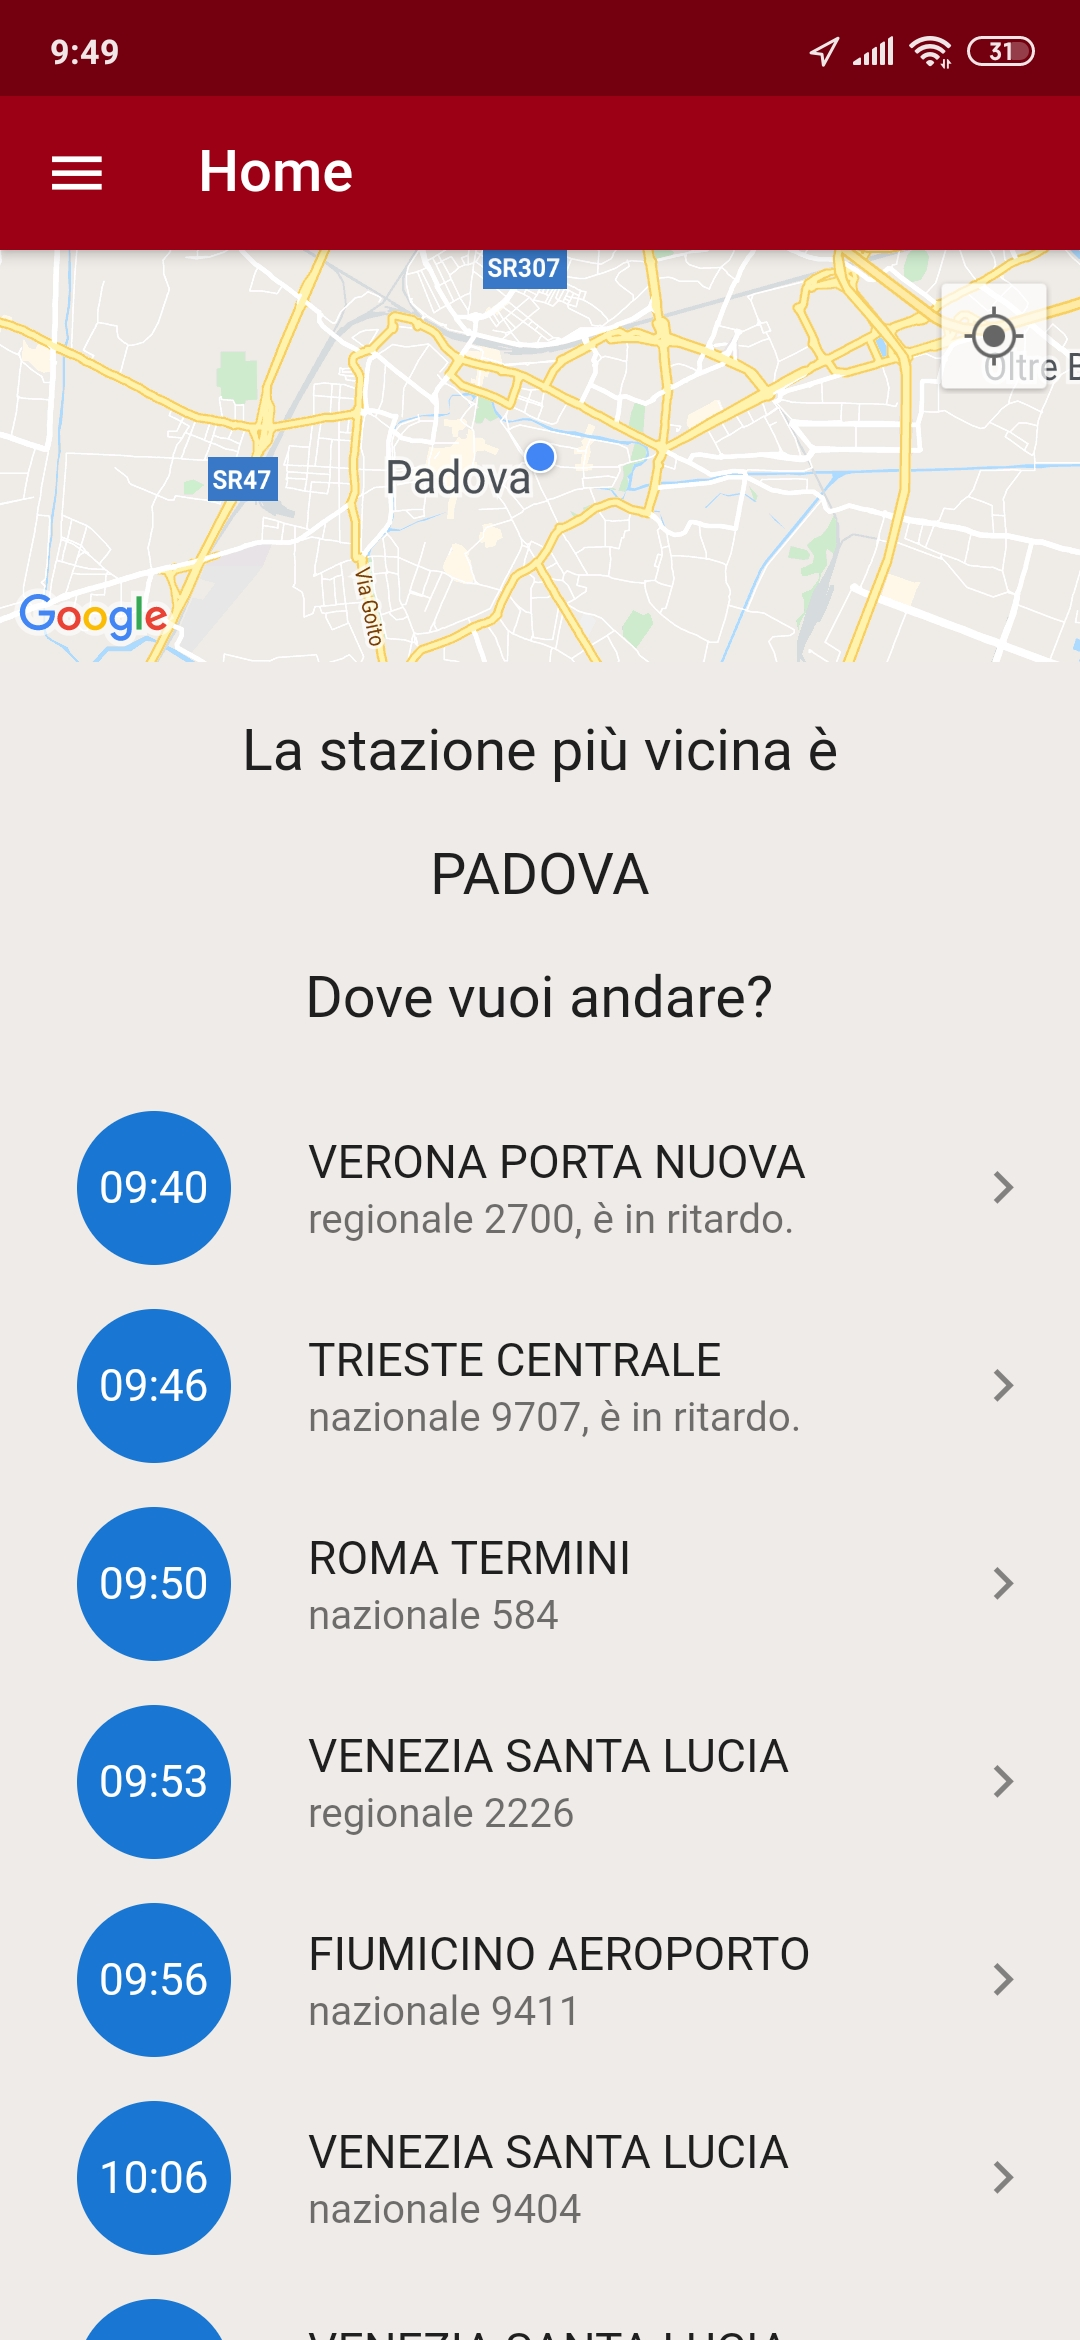
\includegraphics[width=.45\textwidth]{immagini/android/home.jpg}} \quad
    \subfloat[Schermata iOS Home][Schermata iOS Home]
    {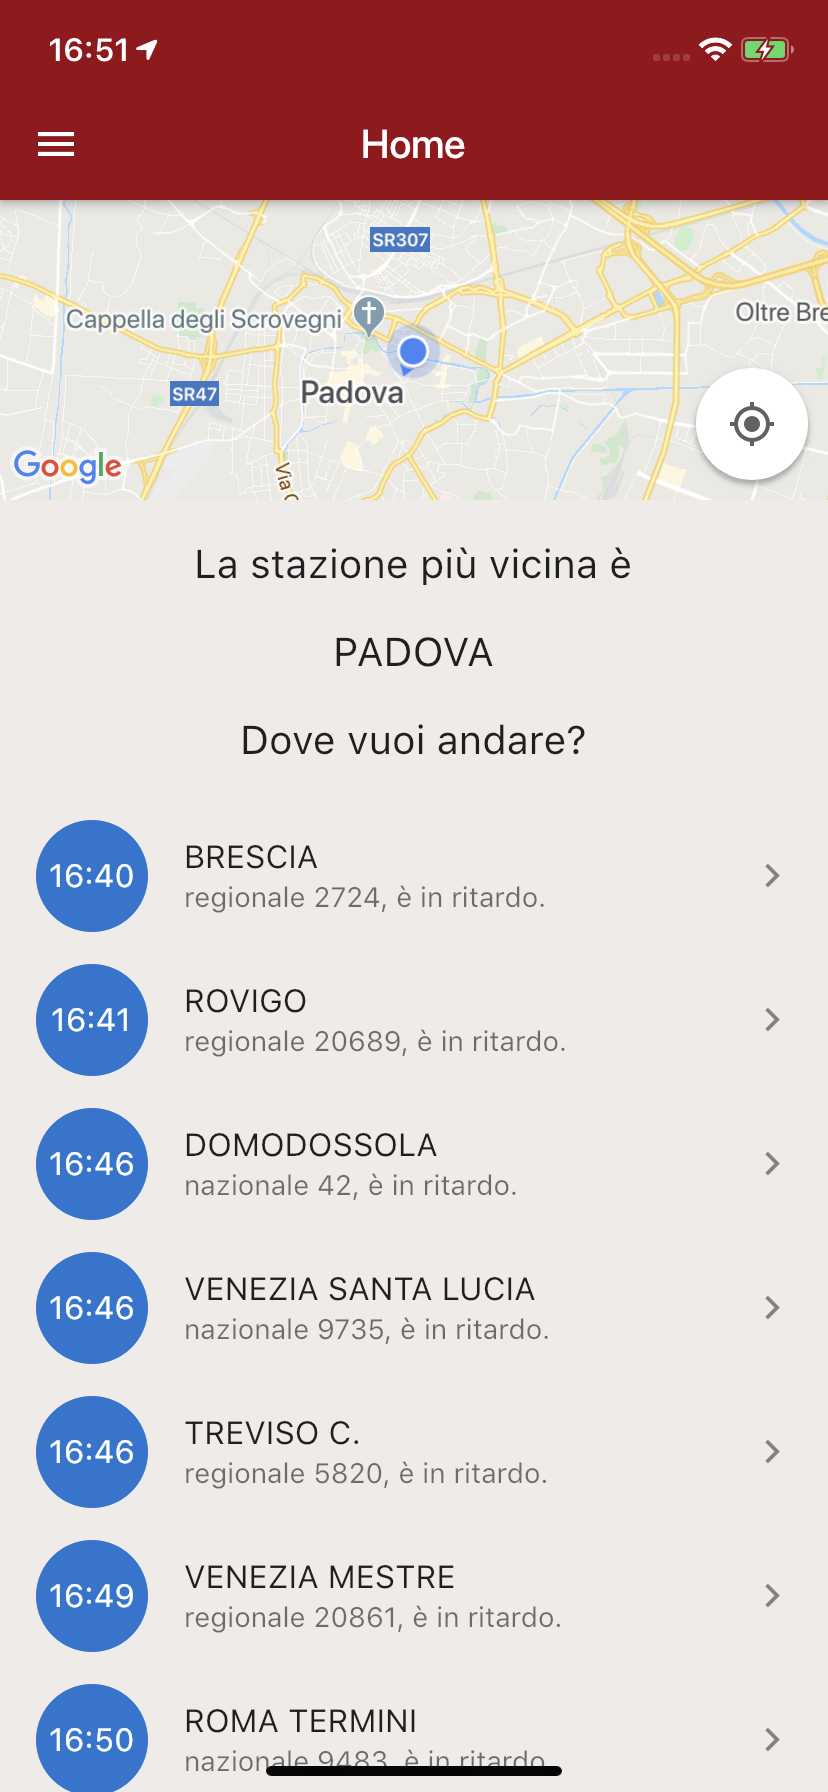
\includegraphics[width=0.45\textwidth]{immagini/ios/home.png}} \quad
    \caption{Schermata Home}
    \label{fig:home}
\end{figure}

Dalla schermata iniziale è possibile vedere la stazione ferroviaria più vicina, localizzata attraverso il GPS.
Viene presentata una lista delle destinazioni raggiungibili tramite i treni in partenza dalla stazione più vicina identificata. Da questa lista di treni è possibile accedere a una pagina con più dettagli relativi al singolo treno.
Questo è un esempio di interfaccia just-in-time che applica la progressive disclosure, perché vengono fornite le informazioni principali relative ai treni in partenza, mentre i dettagli per ognuno di essi possono essere visualizzati attraverso un'ulteriore interazione.

In questa schermata è possibile visualizzare un menù laterale, tramite una gesture di swipe a destra (si veda la sezione~\vref{sec:gesture}). Grazie a questo menù l'utente può raggiungere la pagina relativa al suo profilo, la classifica generale degli utenti, una pagina per rivedere il tutorial per la valutazione di un treno.

\subsection{Stato del treno}

\begin{figure}[htp]
    \centering
    \subfloat[Schermata Android Stato del treno][Schermata Android Stato del treno]
    {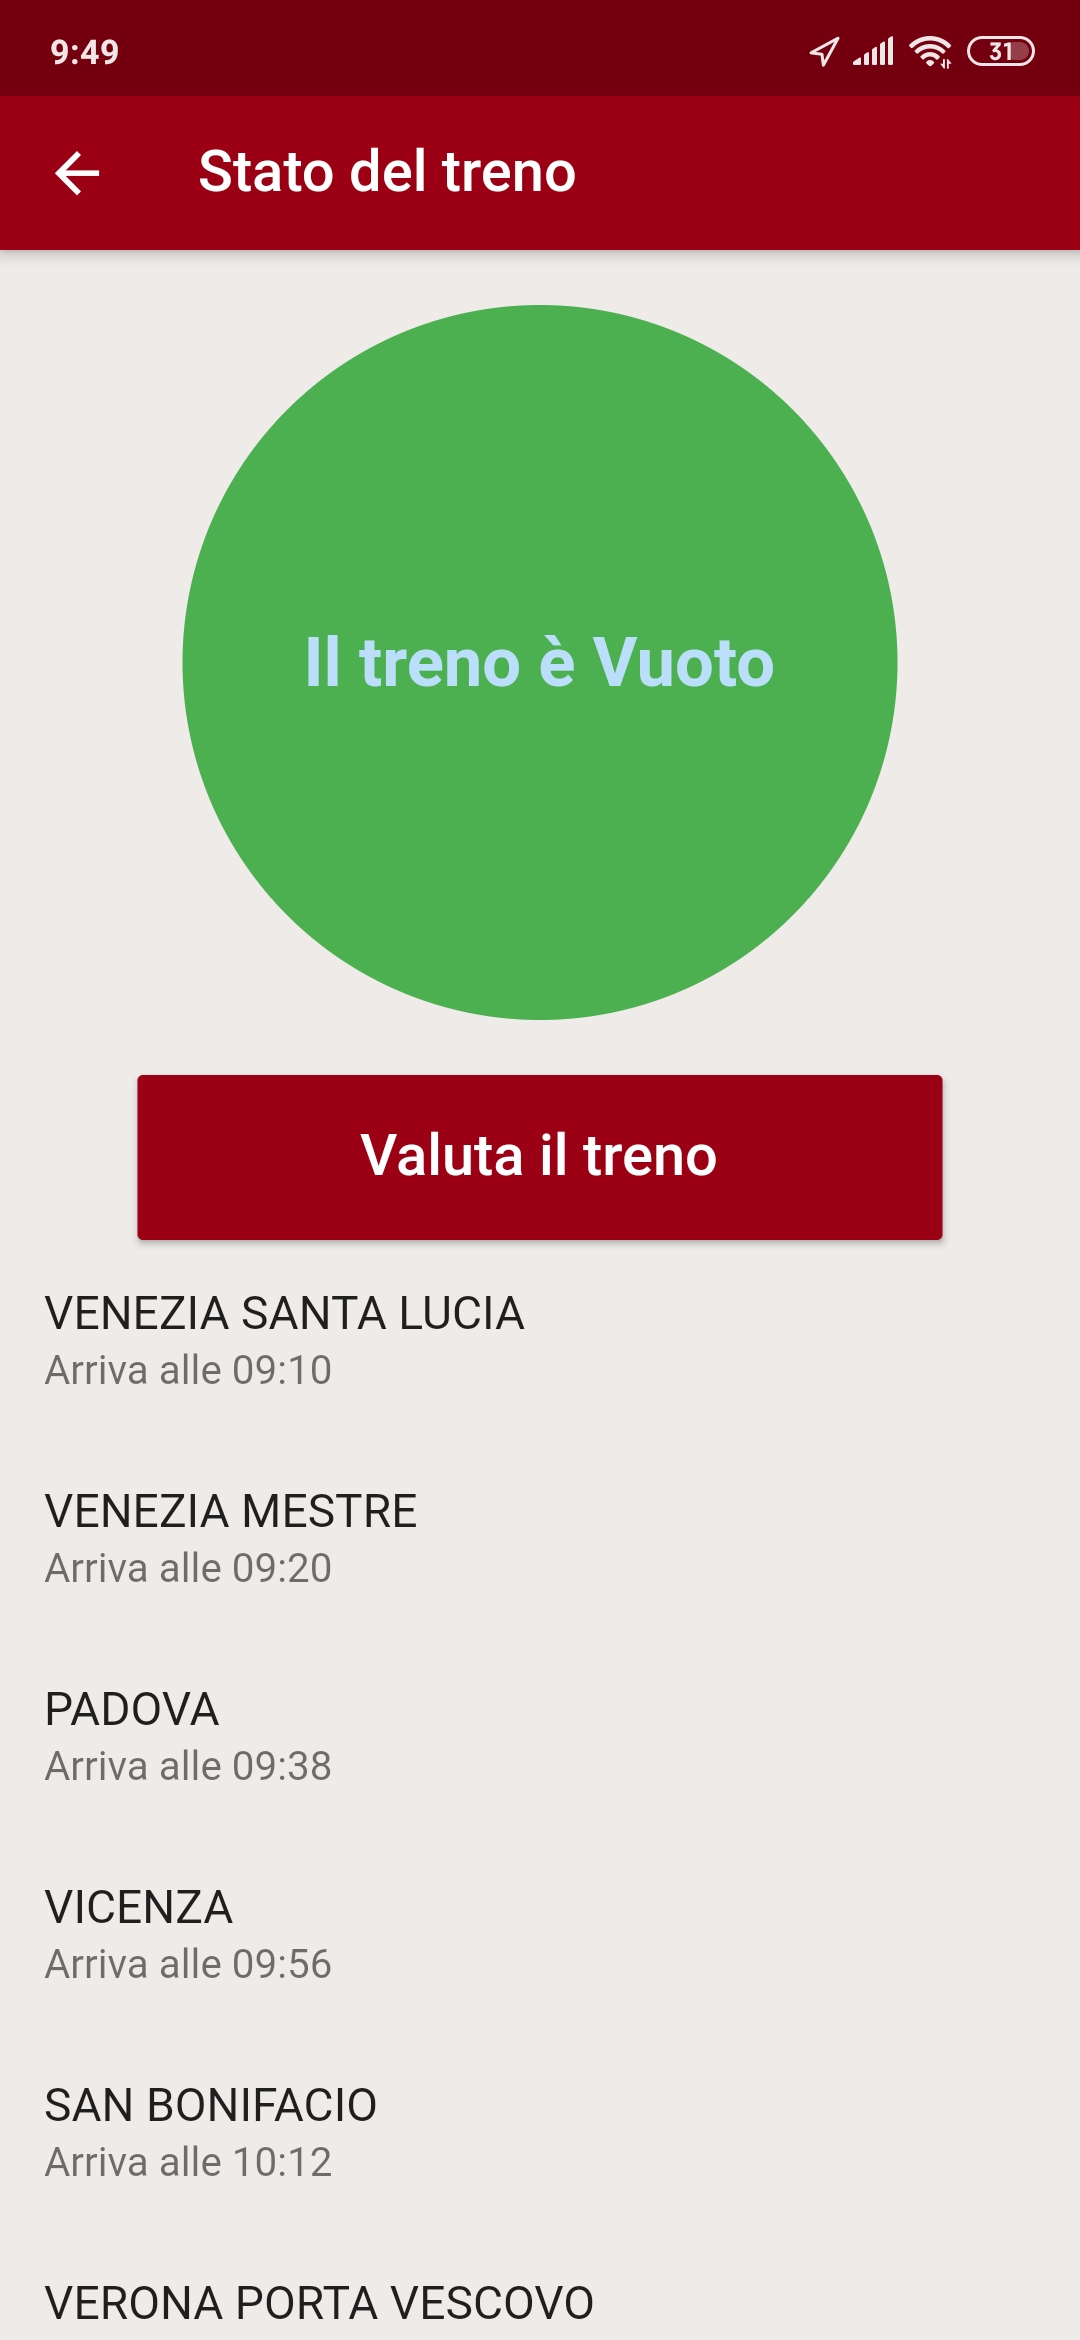
\includegraphics[width=.45\textwidth]{immagini/android/stato.jpg}} \quad
    \subfloat[Schermata iOS Stato del treno][Schermata iOS Stato del treno]
    {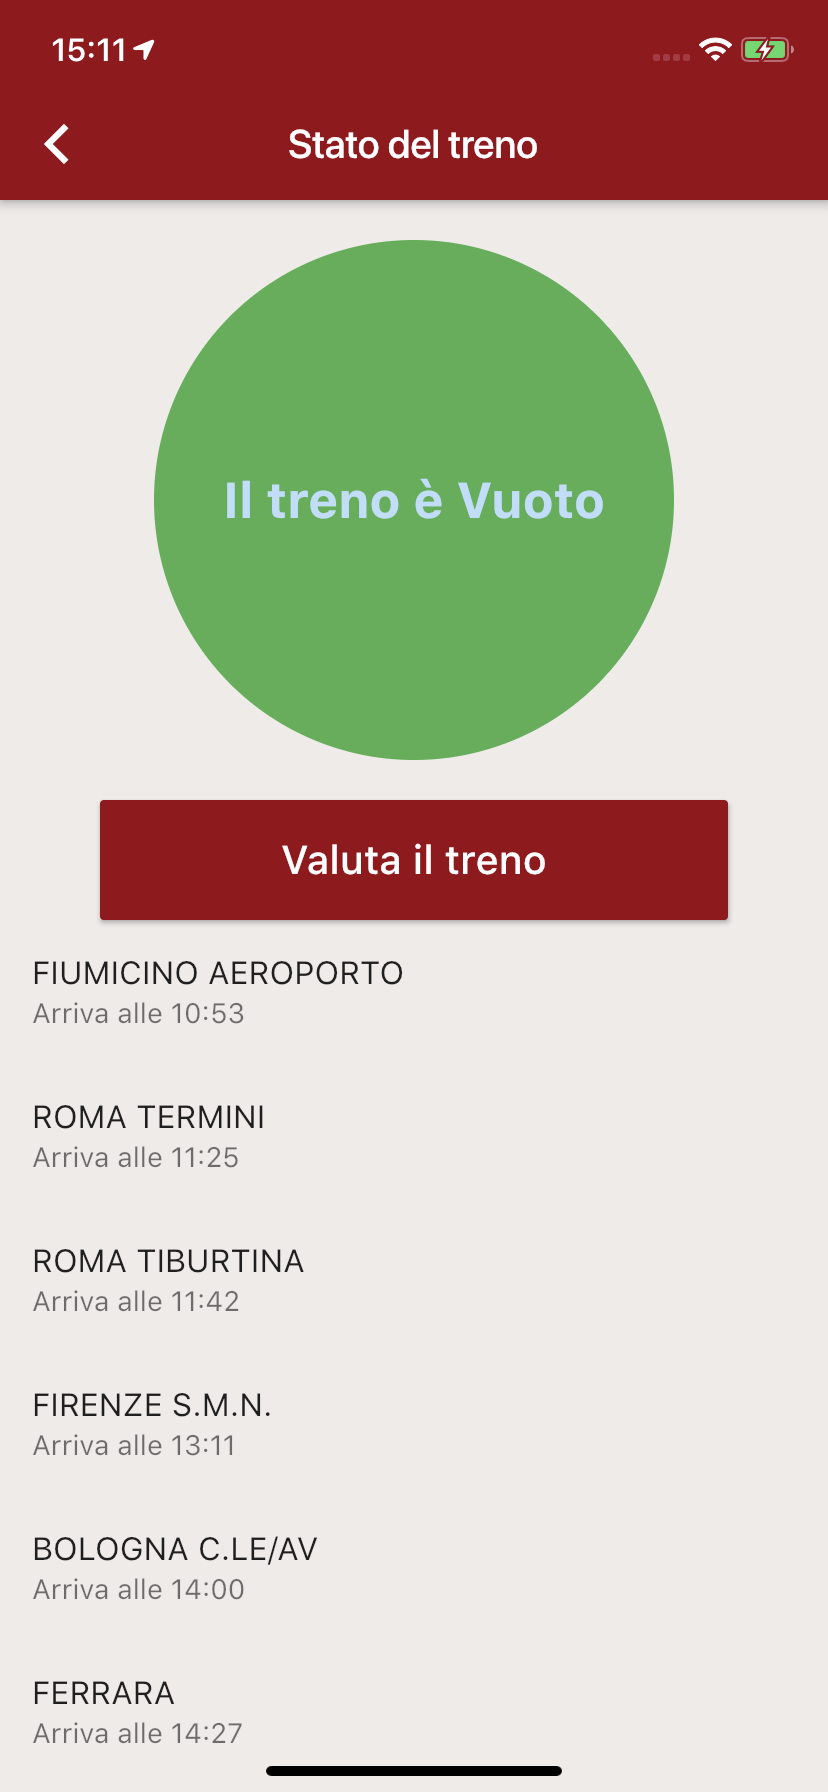
\includegraphics[width=0.45\textwidth]{immagini/ios/stato.png}} \quad
    \caption{Schermata Stato del treno}
    \label{fig:statoTreno}
\end{figure}

In questa schermata l'utente può visualizzare i dettagli del treno selezionato, ovvero la valutazione media assegnata dagli utenti, una lista delle fermate del treno con gli orari di partenza previsti per le diverse fermate e un pulsante per proseguire alla schermata di valutazione del treno.

\subsection{Valuta il treno}

\begin{figure}[H]
    \centering
    \subfloat[Schermata Android Valuta il treno][Schermata Android Valuta il treno]
    {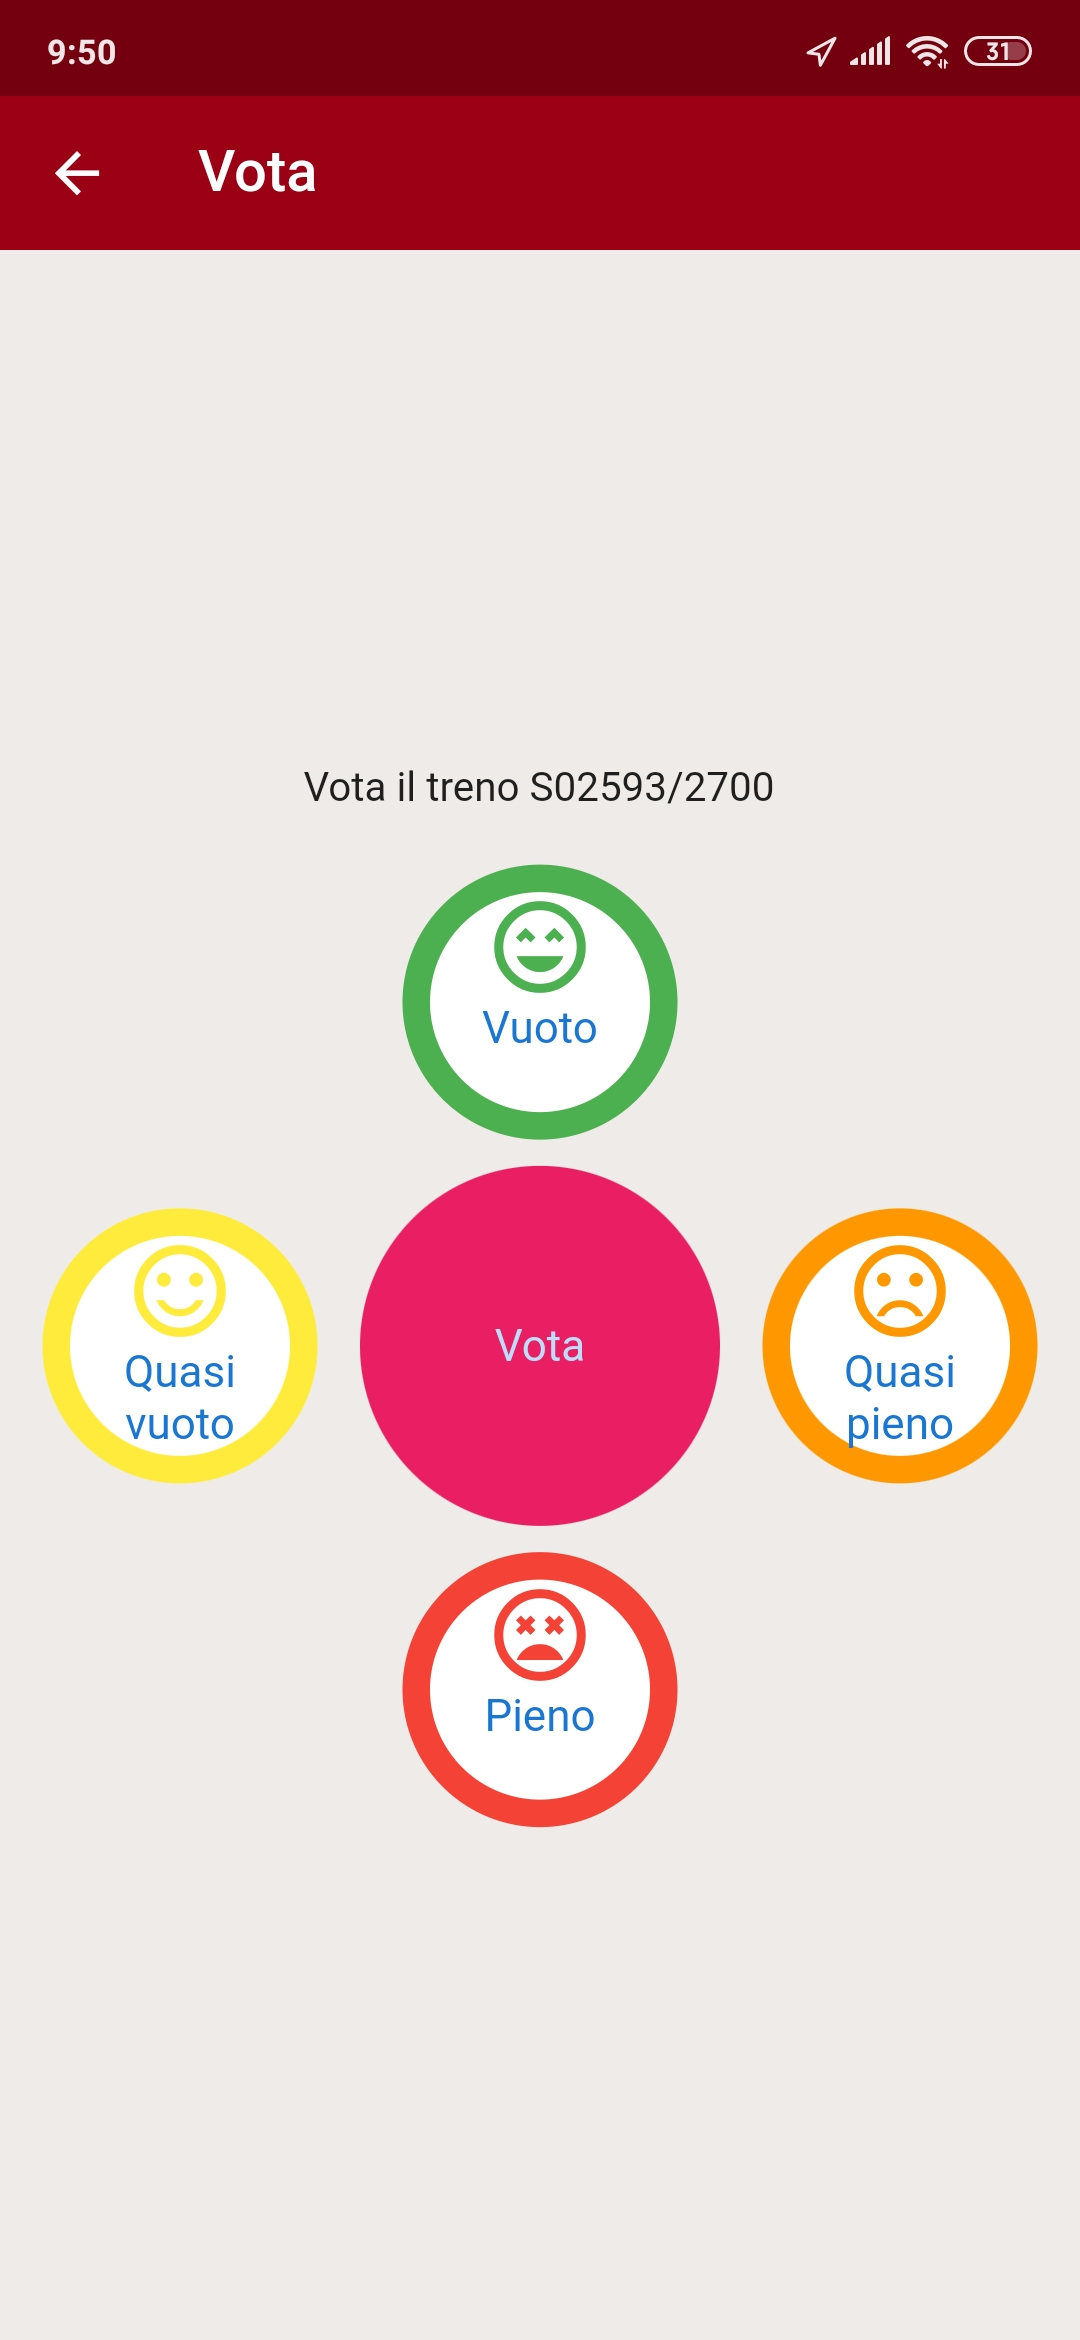
\includegraphics[width=.45\textwidth]{immagini/android/valutazione.jpg}} \quad
    \subfloat[Schermata iOS Valuta il treno][Schermata iOS Valuta il treno]
    {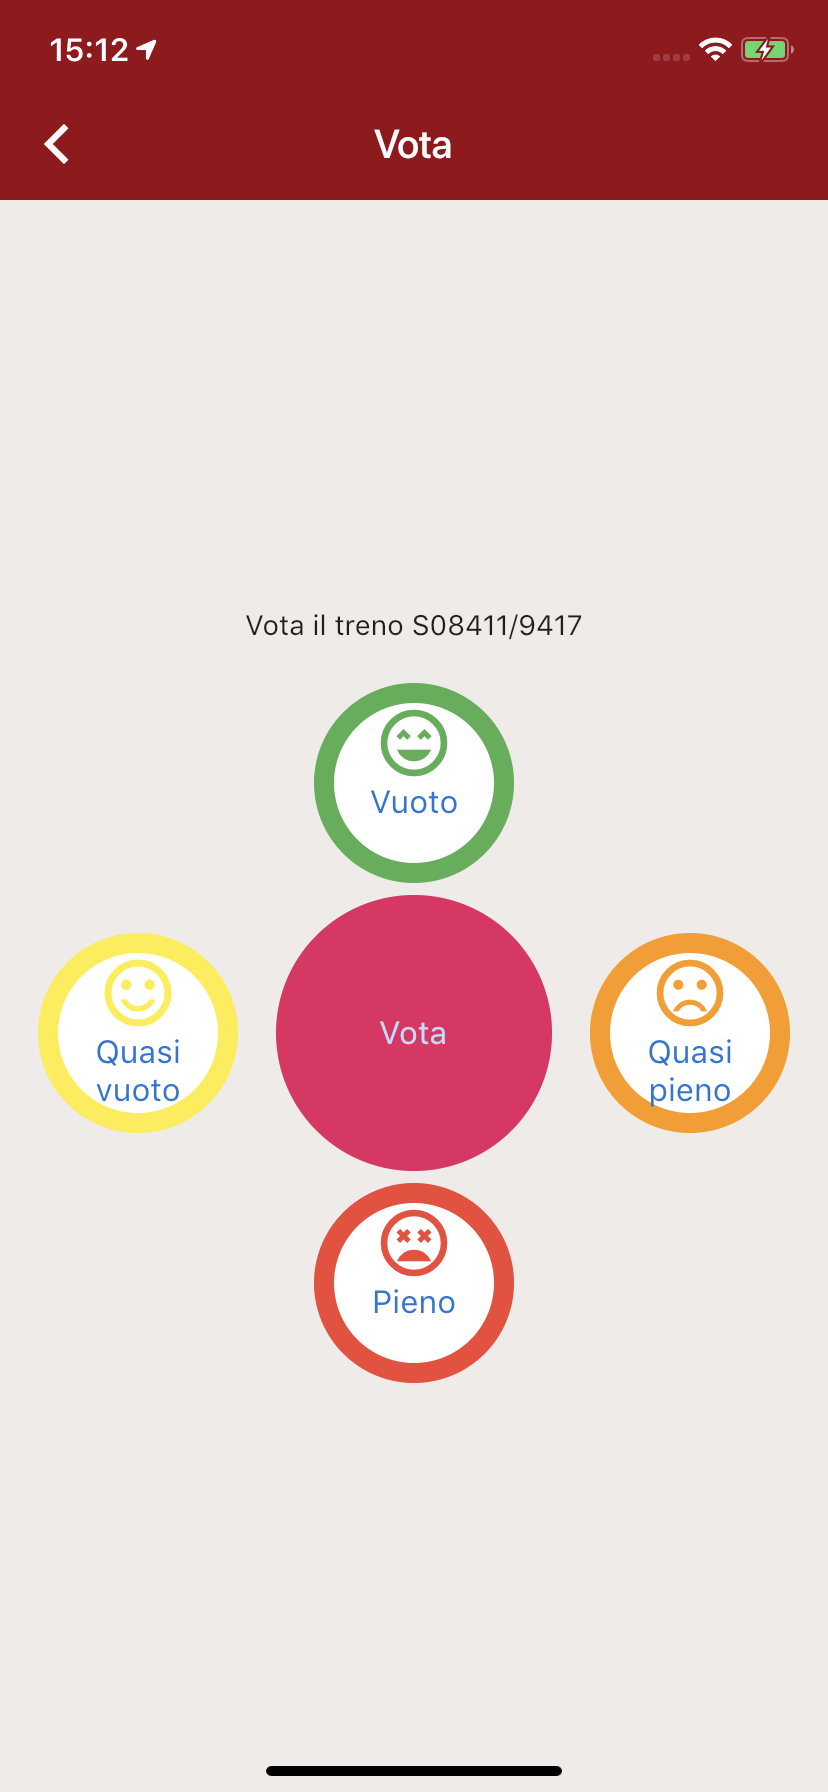
\includegraphics[width=0.45\textwidth]{immagini/ios/valutazione.png}} \quad
    \caption{Schermata Valuta il treno}
    \label{fig:valutaTreno}
\end{figure}

In questa schermata è presente un menù circolare che l'utente dovrà utilizzare per assegnare una votazione al treno, tra le quattro possibili.
Per le prime tre valutazioni all'utente verrà proposto un tutorial veloce per spiegare la gesture di tipo press and drag da utilizzare per la valutazione (si veda la sezione~\vref{sec:gesture}). Una volta eseguita la valutazione l'utente verrà indirizzato alla pagina del profilo per poter visualizzare i suoi punteggi.

\subsection{Hai valutato}

\begin{figure}[H]
    \centering
    \subfloat[Schermata Android Hai valutato][Schermata Android Hai valutato]
    {
\includegraphics[width=.45\textwidth]{immagini/android/haivalutato.jpg}} \quad
    \subfloat[Schermata iOS Hai valutato][Schermata iOS Hai valutato]
    {
\includegraphics[width=0.45\textwidth]{immagini/ios/haivalutato.png}} \quad
    \caption{Schermata Hai valutato}
    \label{fig:haiValutato}
\end{figure}

È stata inserita questa schermata raggiungibile dall'utente solo in seguito ad una votazione. L'aggiunta di tale schermata è stata effettuata per includere all'interno dell'app un elemento di emotional design che potesse suscitare nell'utente un sentimento di gioia e soddisfazione nel vedere la simpatica mascotte dell'applicazione sorridere.

\pagebreak

\subsection{Il tuo Profilo}

\begin{figure}[htp]
    \centering
    \subfloat[Schermata Android Il tuo Profilo][Schermata Android Il tuo Profilo]
    {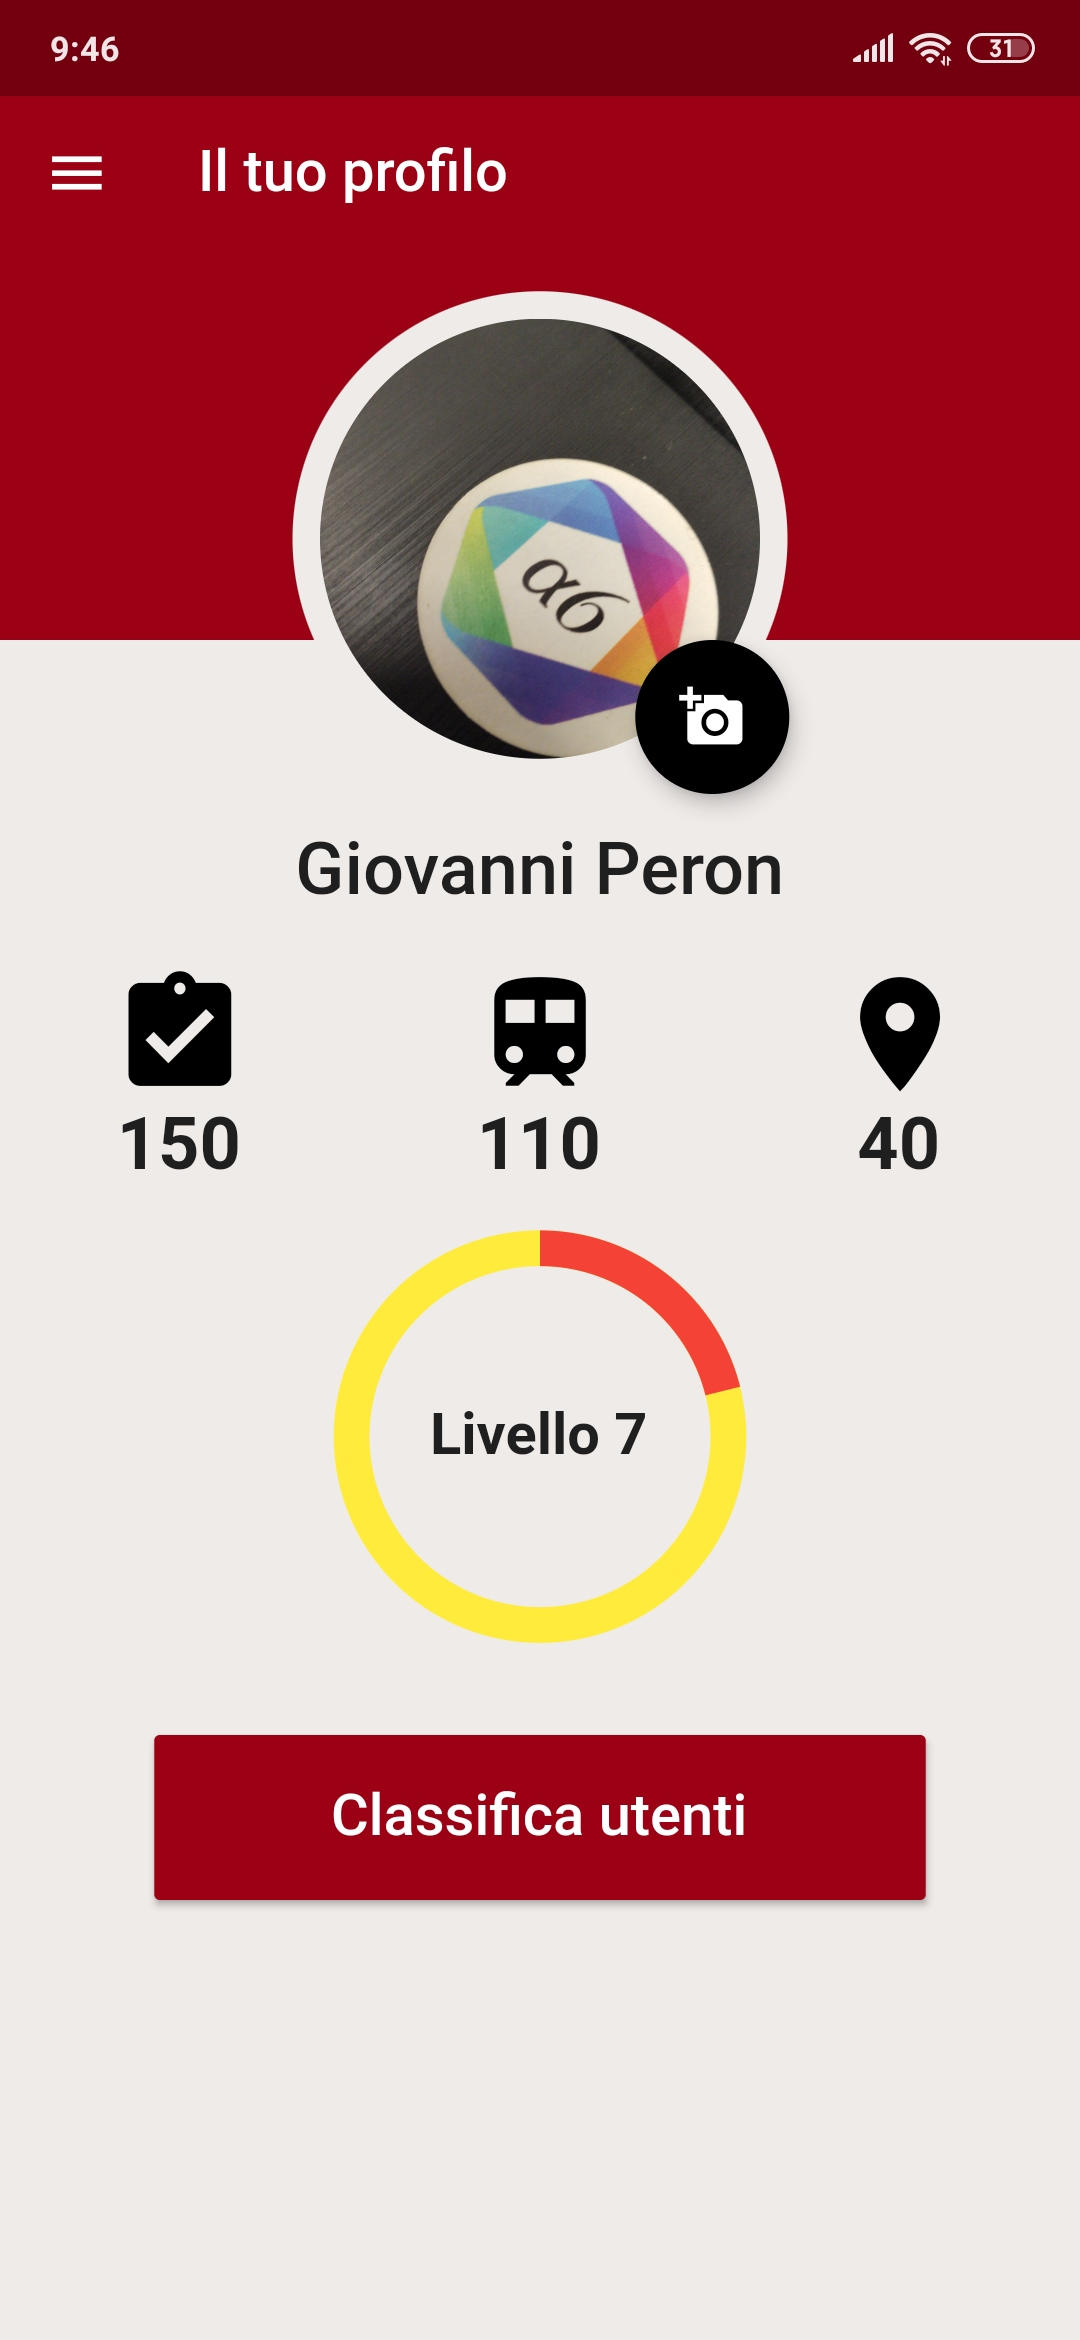
\includegraphics[width=.45\textwidth]{immagini/android/profilo.jpg}} \quad
    \subfloat[Schermata iOS Il tuo Profilo][Schermata iOS Il tuo Profilo]
    {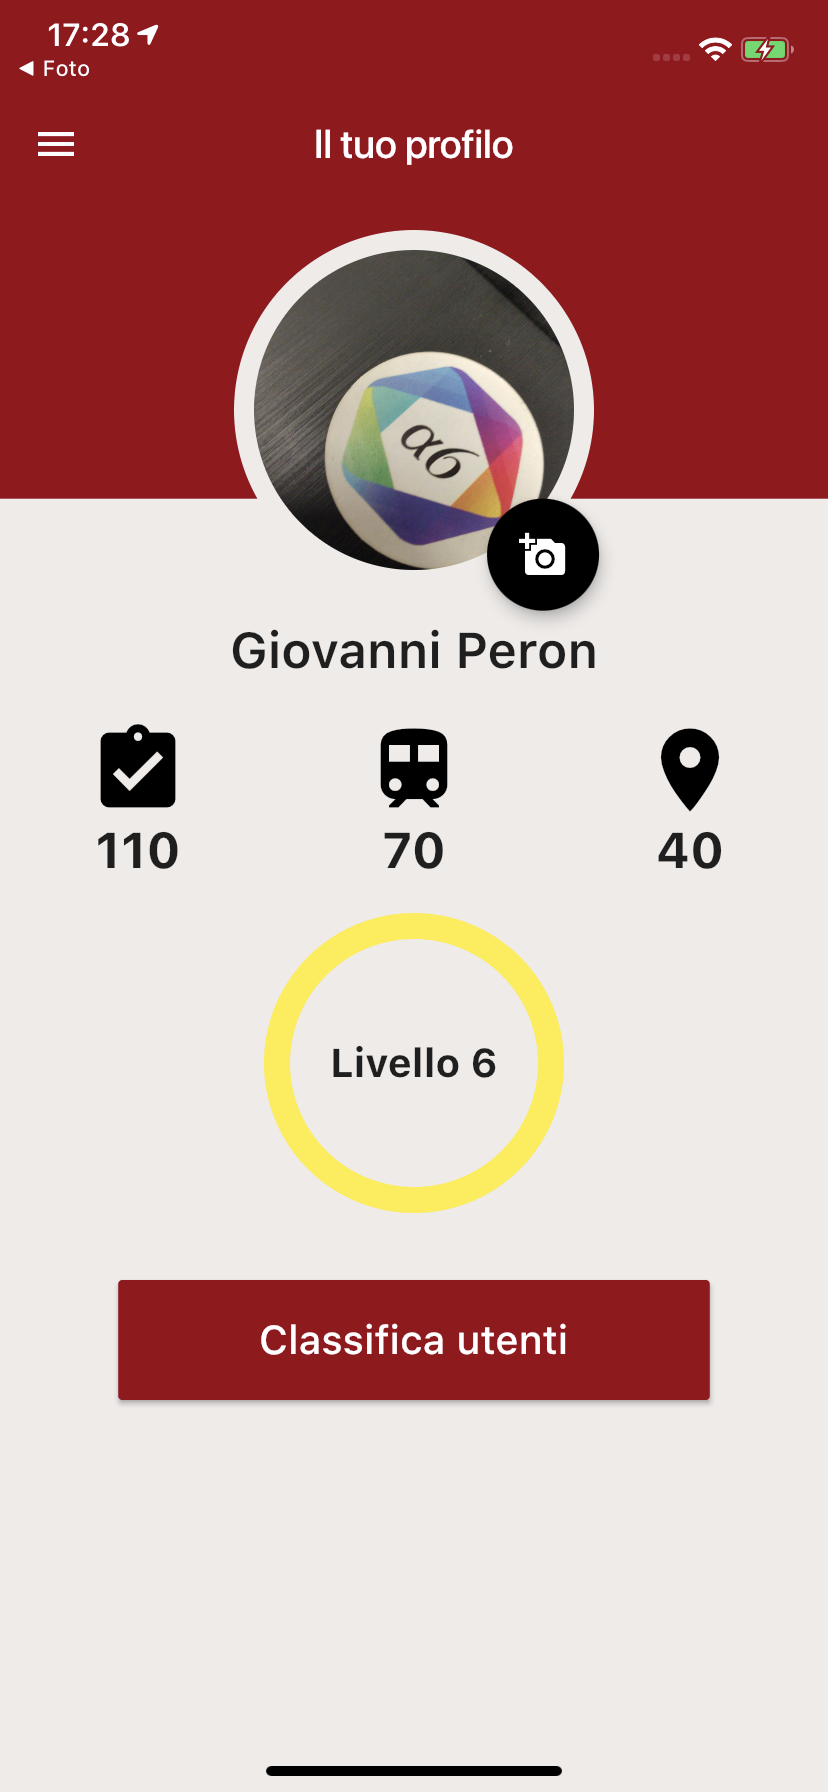
\includegraphics[width=0.45\textwidth]{immagini/ios/profilo.png}} \quad
    \caption{Schermata Il tuo Profilo}
    \label{fig:ilTuoProfilo}
\end{figure}

Nella schermata relativa al profilo, l'utente può visualizzare i suoi dati e i suoi punteggi. Nella parte alta dello schermo è presente l'immagine del profilo modificabile tramite un pulsante posto a lato di essa. Immediatamente sotto al nome del proprio account l'utente può visualizzare i punteggi relativi alle valutazioni eseguite, il numero di treni differenti valutati, e il numero di valutazioni eseguite da stazioni differenti. È presente inoltre un pulsante per poter accedere alla classifica generale.

\pagebreak

\subsection{Informazioni}

\begin{figure}[htp]
	\centering
	\subfloat[Schermata Android Informazioni][Schermata Android Informazioni]
	{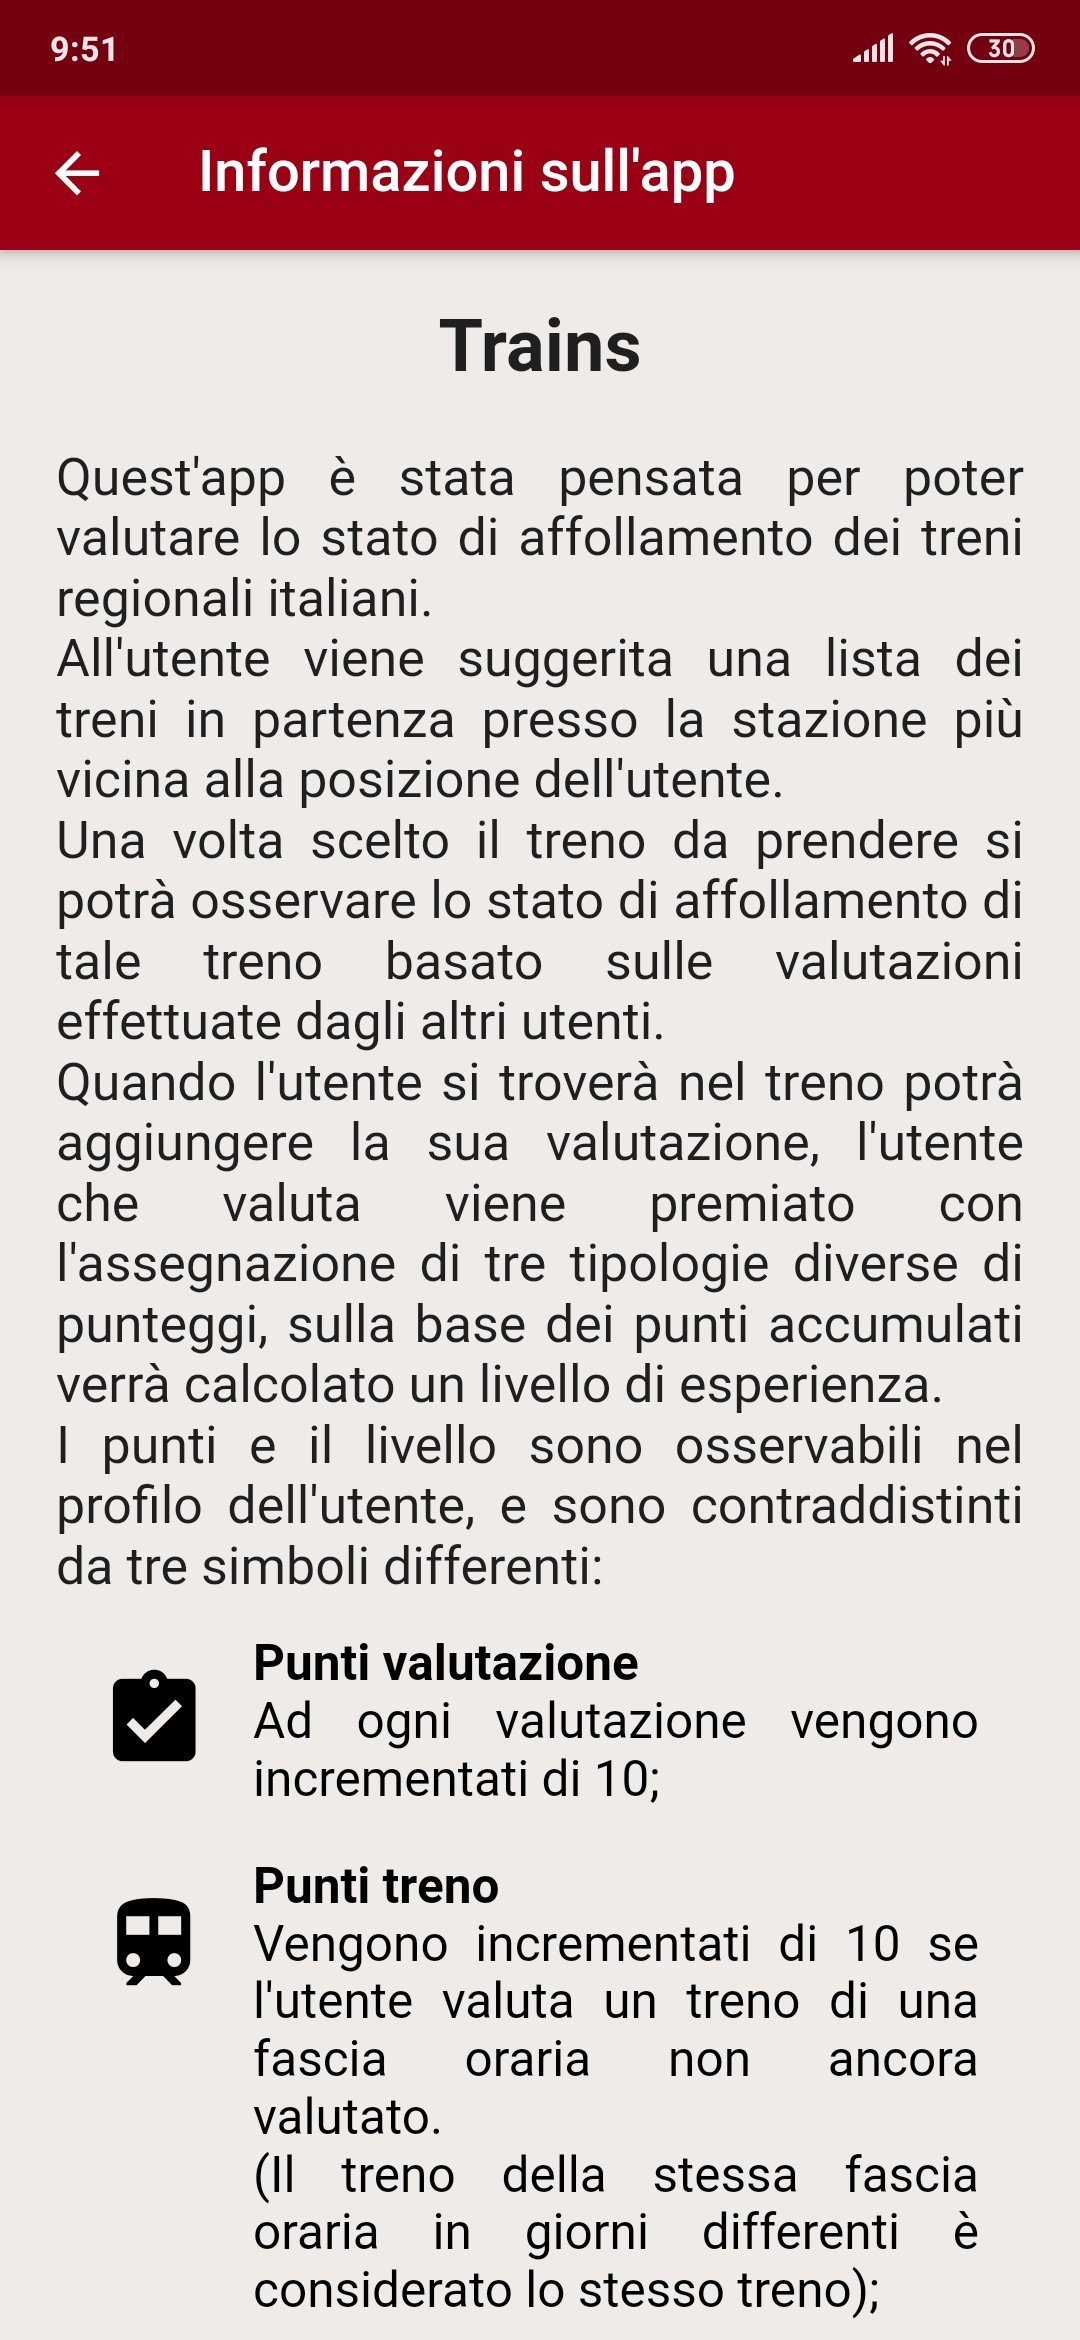
\includegraphics[width=.45\textwidth]{immagini/android/informazioni.jpg}} \quad
	\subfloat[Schermata iOS Informazioni][Schermata iOS Il tuo Informazioni]
	{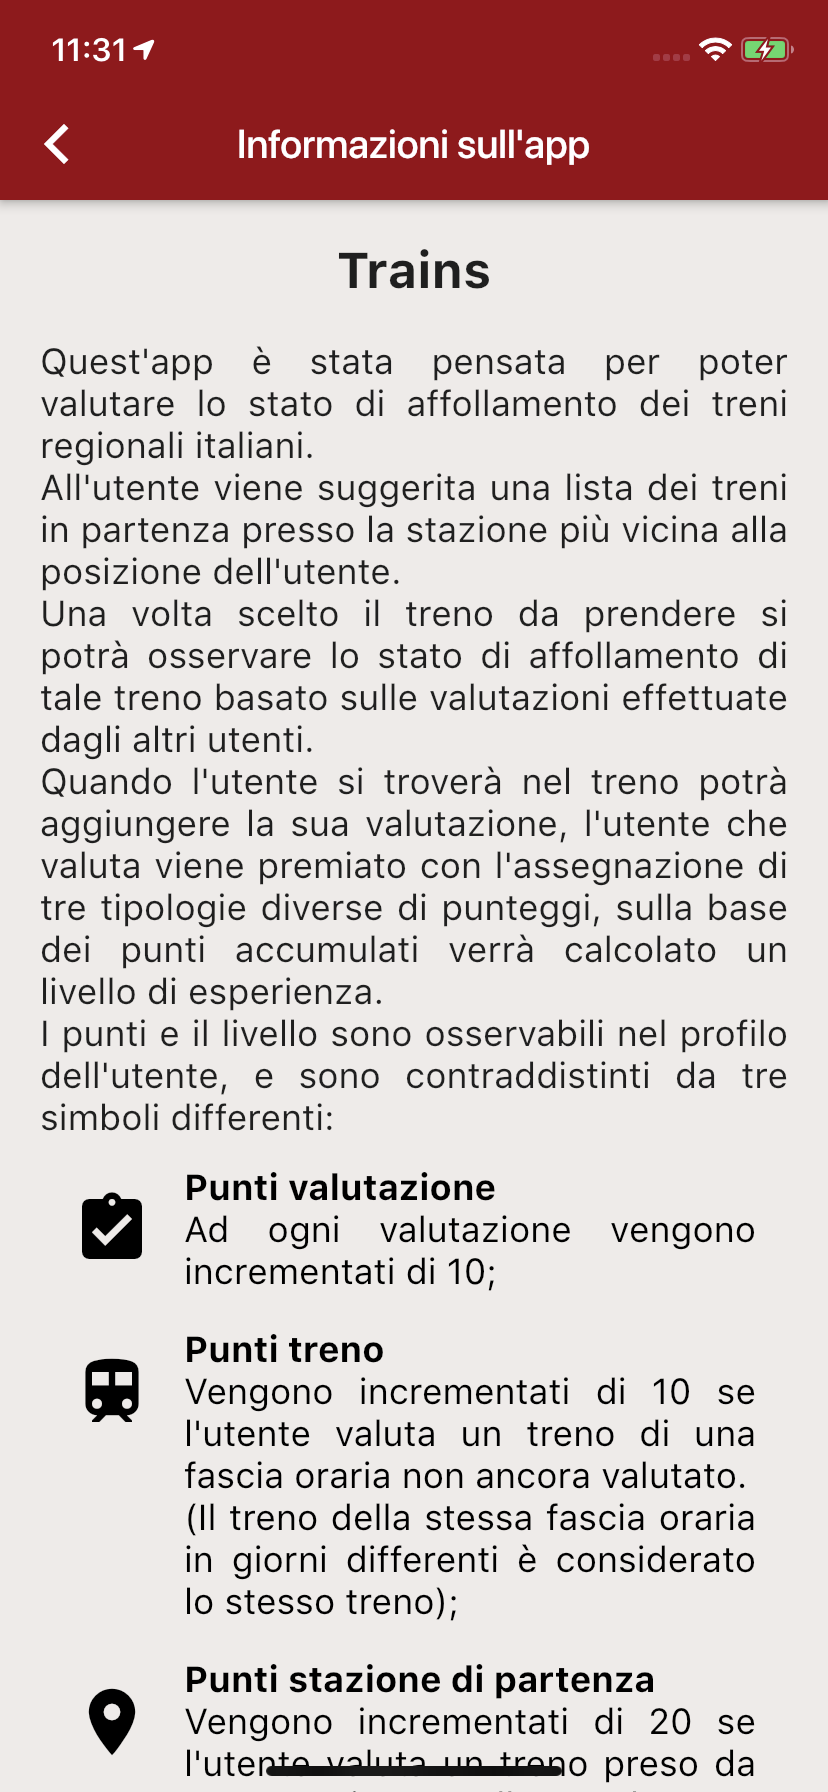
\includegraphics[width=0.45\textwidth]{immagini/ios/informazioni.png}} \quad
	\caption{Schermata Informazioni}
	\label{fig:Informazioni}
\end{figure}

È stata inclusa una schermata contenente una descrizione dell'applicazione e le informazioni di base che l'utente deve sapere per poterla utilizzare. Sebbene queste informazioni dovrebbero risultare molto intuitive per l'utente è stato comunque pensato di aggiungere questa pagina per venire incontro agli utenti nel caso questi possano avere dubbi o non comprendere appieno il significato di qualche simbolo. In alternativa avremmo potuto utilizzare messaggi just-in-time ma è stata preferita questa soluzione per evitare messaggi troppo lunghi e per non interrompere troppo frequentemente l'esperienza dell'utente.

\pagebreak

\section{Gesture utilizzate\label{sec:gesture}}

\subsection{Gesture menù laterale}
Per accedere al menù laterale evitando di inserire pulsanti è stato scelto di utilizzare una gesture di swipe a destra. Questo tipo di gesture è stata scelta perché consente all'utente di visualizzare il menù laterale tramite un gesto effettuabile dal lato sinistro della comfort zone, quindi sicuramente più comodo rispetto a un pulsante che avrebbe potuto prendere posizione nella parte alta dello schermo, e non in quella bassa per non creare uno stack di pulsanti in Android \parencite{gaggi:mobileDesign}.

\subsection{Gesture valutazione treno}
Lo strumento per la valutazione del treno è stato realizzato attraverso un menù circolare, da cui è possibile fornire quattro voti. La votazione viene effettuata tramite una gesture press and drag che consente all'utente di scegliere il voto desiderato trascinando il simbolo corrispondente ad esso al centro dello schermo. 
Questa scelta vincola la disposizione e il numero delle opzioni del menù che non saranno più modificabili in futuro, perché si andrebbero a rompere le convenzioni che si creano con l'utente, tuttavia l'utilizzo di una gesture rende molto più veloce ed istantaneo il processo di valutazione del treno che è l'aspetto più importante dato che ipotizziamo che l'utente esegua tale l'azione in un ambiente precipitoso, frettoloso, come una stazione o un treno.   

È stato scelto questo tipo di trascinamento dall'esterno all'interno perché, anche se forse potrebbe risultare meno comune rispetto allo spostamento verso l'esterno dello schermo, è stato pensato che il trascinamento verso l'interno può diminuire la probabilità di commettere errori. Presentare un unico oggetto centrale trascinabile verso l'esterno avrebbe reso la votazione dipendente dalla direzione del gesto data dall'utente (verso l'alto, il basso, a destra o a sinistra), mentre il fatto di dover prima scegliere l'oggetto e poi eseguire il trascinamento verso il centro dello schermo, consente di prestare più attenzione alla scelta del voto ed elimina la dipendenza dalla direzione della gesture che può essere facilmente sbagliata dall'utente per la fretta del gesto o per poca manualità. 

Sono state scelte quattro valutazioni possibili, il numero di voti disponibili è volutamente pari per evitare che l'utente possa scegliere sempre un valore neutrale centrale, evitando quindi di pensare alla valutazione che sta esprimendo. 
Per i primi tre voti espressi dall'utente, viene fornito un tutorial just-in-time per fornire poche semplici istruzioni su come votare il treno su cui si è saliti.
Dopo i tre voti il tutorial sparisce, pur restando raggiungibile dal menù laterale.